\documentclass[]{scrartcl}

\usepackage[utf8]{inputenc}
\usepackage{amsmath}
\usepackage{amssymb}
\usepackage{amsthm}
\usepackage{setspace}
\usepackage{graphicx}
\usepackage[dvipsnames]{xcolor}
\usepackage[%
colorlinks = true,
citecolor  = RoyalBlue,
linkcolor  = RoyalBlue,
urlcolor   = RoyalBlue,
unicode,
]{hyperref}
% introduces some common math macros
\newcommand{\diff}{\mathrm{d}}
\newcommand{\calg}{\mathcal{G}}
\newcommand{\calb}{\mathcal{B}}
\newcommand{\calf}{\mathcal{F}}
\newcommand{\bbf}{\mathbb{F}}
\newcommand{\bbp}{\mathbb{P}}
\newcommand{\R}{\mathbb{R}}
\newcommand{\E}{\mathbb{E}}
\newcommand{\hatpsi}{\widehat{\psi}}
\newcommand{\tol}{\mathsf{tol}}
%macro for a comment from JP
\newcommand{\cjp}[1]{{\color{orange}[JP] #1}}

%%%%%%%%%%%%%%%%%%%%%%%%%%%%%%%%%%%%%%%%
%
% tikz stuff
%
%
%%%%%%%%%%%%%%%%%%%%%%%%%%%%%%%%%%%%%%%%
\usepackage[utf8]{inputenc}
\usepackage{pgfplots}
%\DeclareUnicodeCharacter{2212}{−}
\usepgfplotslibrary{groupplots,dateplot}
\usetikzlibrary{patterns,shapes.arrows}
\pgfplotsset{compat=newest}
\pgfplotsset{compat=1.13}
\usepgfplotslibrary{fillbetween}
\pgfmathdeclarefunction{gauss}{2}
{\pgfmathparse{1/(#2*sqrt(2*pi))*exp(-((x-#1)^2)/(2*#2^2))}}
%symbol definitions
\pgfplotsset{
	colormap/viridis,
}
%\usepgfplotslibrary{colorbrewer} % LATEX and plain TEX
%\usepgfplotslibrary[colorbrewer] % ConTEXt
%\usetikzlibrary{pgfplots.colorbrewer} % LATEX and plain TEX
%\usetikzlibrary[pgfplots.colorbrewer] % ConTEXt
%%%%%%%%%%%%%%%%%%%%%%%%%%%%%%%%%%%%%%%%
\usepackage{booktabs}
%should be last to not create conflicts
\usepackage{hyperref}
\usepackage{cleveref}
\usepackage{autonum}
\usepackage{algorithm}
\usepackage{algpseudocode}
\usepackage{algorithmicx}
\usepackage{bm}
% Title Page
\title{Data report  for Drift}
\author{Juan Pablo Madrigal Cianci}


\begin{document}
	\maketitle
	
	\begin{abstract}
	\end{abstract}
	\section{Dataset and overall behaviour}
	
	We focused our analysis on the \texttt{SOL-PERP} market dataset. At the time of writing, such a dataset contained information about  \textbf{984906} different trades from 2022-01-01 at 00:00:14.251 to 2022-04-24 at 18:29:45.983 with a total volume of 1'652,486,950.65 USD ($\approx$ 1.65 Bn. USD). The codes used to recreate the presented figures are available upon request.  We begin with a simple exploratory data analysis presented in Table \ref{tab:1}. There, we show the mean, standard deviation, and quantiles of several quantities of interest. In particular, \texttt{Base} represents the amount of base asset, \texttt{Quote} represents the amount of quote asset, \texttt{Oracle} and \texttt{Mark} are the oracle and mark price, respectively, $\Delta t$ measures the amount of time, in seconds, between any two transactions, and \texttt{Longs}, \texttt{Shorts} are the amount of open shorts and long positions (total open - liquidations). 
	
	\begin{table}[H]\scriptsize{
			\begin{tabular}{@{}lllllllll@{}}
				\toprule
				& Base   & Quote  & Fee        & Oracle  & Mark      & $\Delta t$         & Shorts & Longs  \\ \midrule
				mean & 15.995 & 1675.045 & 1.666 & 107.358 & 107.498 & 9.981  & 238889.304 & 239338.805  \\
				standard deviation  & 29.411 & 3092.325 & 3.055 & 20.744  & 20.784  & 43.506 & 139637.943 & 140053.162 \\
				min  & 0.000  & 0.000    & 0.000 & 75.626  & 6.188   & 0.000  & 0.000      & 1.000      \\
				25\% & 3.201  & 341.575  & 0.335 & 91.510  & 91.639  & 0.167  & 115924.000 & 116335.250  \\
				50\% & 9.287  & 998.906  & 0.999 & 101.609 & 101.686 & 1.462  & 236150.000 & 240759.500  \\
				75\% & 18.995 & 1963.428 & 1.956 & 117.028 & 117.112 & 5.986  & 360902.000 & 360043.750  \\
				max & 10873.000       & 953964.173       & 953.964 & 179.479     & 948.967   & 23503.333  & 480599.000  & 484821.000 
		\end{tabular}}
		\caption{Summary statistics for the $\texttt{SOL-PERP}$ dataset. \label{tab:1}}
	\end{table}
	
	
	
	
	\subsubsection*{On the distribution of quote amount and $\Delta t$} From table \ref{tab:1} it can see that for Quote and $\Delta t$, the standard deviation is much larger than the mean, and that the median (50\% quantile) is much smaller than the mean, which suggests that the distributions of these quantities heavily skew to the right. This is further verified in Figure \ref{fig:densdt} where we plot the histogram of the natural logarithm of these quantities. We remark that we decided to take the logarithm for ease of visualization since the range of these values spans several orders of magnitude. It can furthermore be seen that the distribution of $\log(\Delta t)$ seems to be bi-modal, meaning that the number of times between transactions concentrates around two different values. Furthermore, the plots in Figure \ref{fig:trace}  indicate that there is no visible trend for either of these values, indicating stationarity (with respect to time). This suggests that one could model the arrival times $\Delta t$ and the (quote) transaction amounts by fitting a probability distribution to these values via, e.g., a Kernel Density Estimator (KDE). This is important in the sense that, one could use those samples to create realistic simulators too, e.g., backtest the efficiency of proposed changes to the fee mechanism. 
	
	\begin{figure}
		\centering
		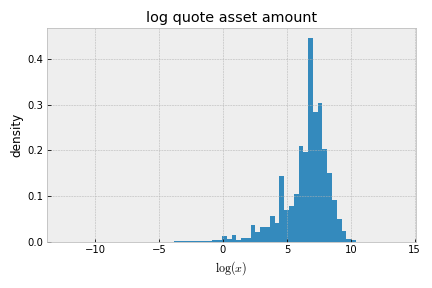
\includegraphics[width=0.47\linewidth]{figures/dens_quote}
		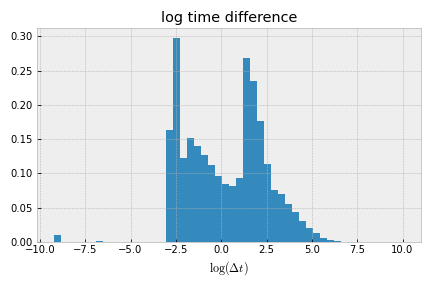
\includegraphics[width=0.47\linewidth]{figures/dens_dt}
		\caption{Histograms for the amount of quote asset (USD) of each transaction (left), and for the time (in seconds) between transactions. (right). }
		\label{fig:densdt}
	\end{figure}
	
	\begin{figure}
		\centering
		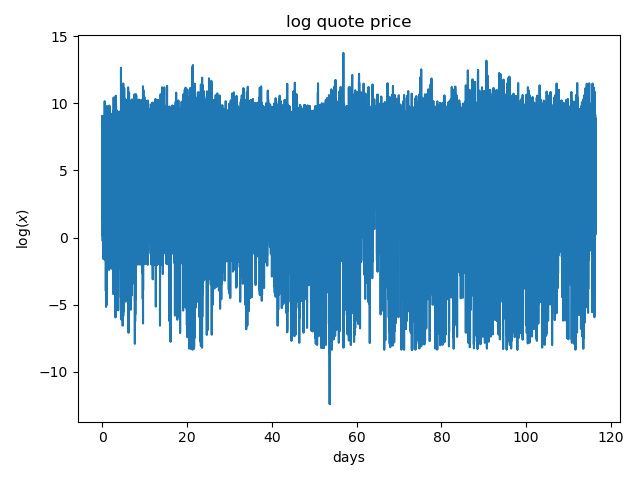
\includegraphics[width=0.47\linewidth]{figures/dxvst}
		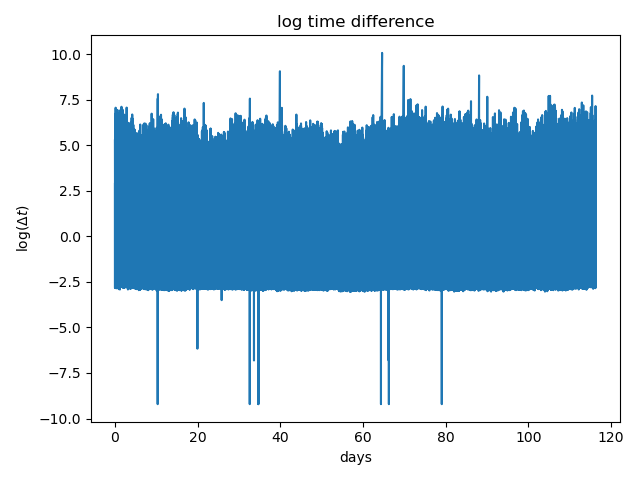
\includegraphics[width=0.47\linewidth]{figures/dtvst}
		
		\caption{Amount of quote asset (USD) of each transaction vs time (left), and time (in seconds) between transactions vs time (right). }
		\label{fig:trace}
	\end{figure}
	
	
	
	\subsubsection*{Parity of long-short positions} Table \ref{tab:1} also suggests some sort of long-short parity; i.e., that, over time, the amount of open long positions closely resembles the amount of short positions opened. This is further evidenced in Figure \ref{fig:lts} where we plot the long-to-shorts ratio.  The fact that there's an approximately equal amount of open long and shorts positions is indicative of a healthy market and pricing mechanism.
	
	
	
	
	\begin{figure}
		\centering
		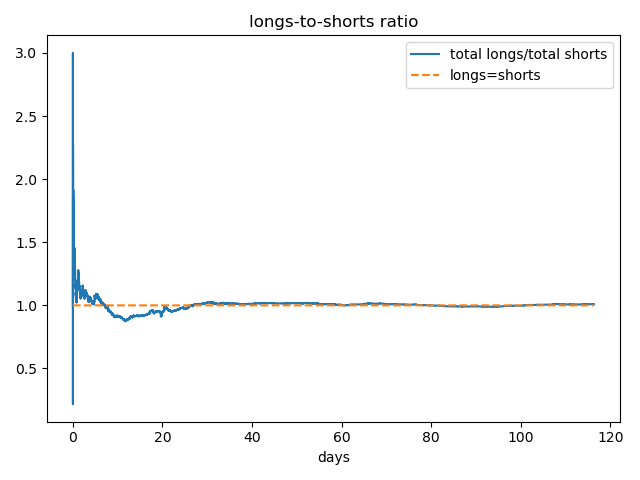
\includegraphics[width=0.47\linewidth]{figures/lts}
		\caption{Long-short ratio.}
		\label{fig:lts}
	\end{figure}
	
	
	\subsubsection*{Measuring arbitrages} 
	Due to the inner workings of (v)AMMs, it will in general be the case that the mark price and the oracle price of a given asset will be  different from each other. It is well-known that this in turn leads to arbitrage opportunities in the DEX.  We now classify transactions into arbitrages or not. Given some $\alpha\in[0,1)$, we say that a transaction was an \emph{$\alpha$-arbitrage} if  either one of (i) or (ii) are satisfied: \begin{enumerate}
		\item[(i)] Transaction  direction is \texttt{Long} and \texttt{Mark}<$(1-\alpha)$\texttt{Oracle} .
		\item[(ii)] Transaction direction is  \texttt{Short} and \texttt{Mark}>$(1+\alpha)$\texttt{Oracle}. 
	\end{enumerate}
	Notice that (i) can be understood as buying an asset with a discount of $(100\times\alpha)$\% with respect to the oracle price. Conversely, (ii) is equivalent to selling an asset with a price increase of $(100\times \alpha)$\%. We use this definition to classify whether the trades are an $\alpha$-arbitrage or not, for different values of  $\alpha=\{0,0.005,0.01\}$. We present our results in Figure \ref{fig:piearb0}. Notice that at $\alpha=0$,  the majority of transactions are classified as arbitrage. Given that the ratio between long and shorts is approximately 1,  this information suggests that there might be a systematic misprice of the mark price. We will discuss this in further detail in Section \ref{sec:oracle}. Notice, however, that once one considers larger values of $\alpha$, the proportion of $\alpha$ arbitrages rapidly decreases.
	
	
	\begin{figure}
		\centering
		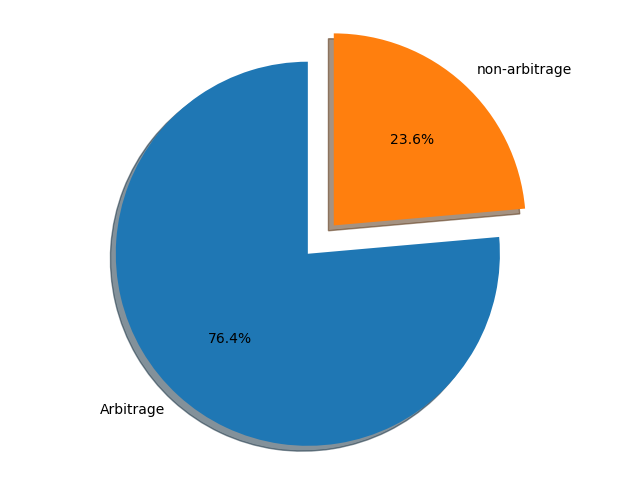
\includegraphics[width=0.32\linewidth]{figures/pie_arb00}
		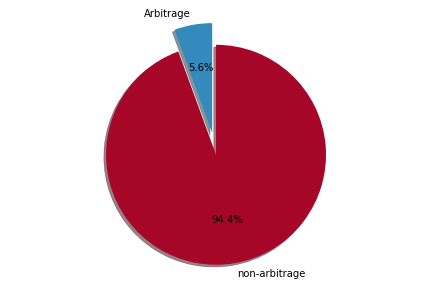
\includegraphics[width=0.32\linewidth]{figures/pie_arb05}
		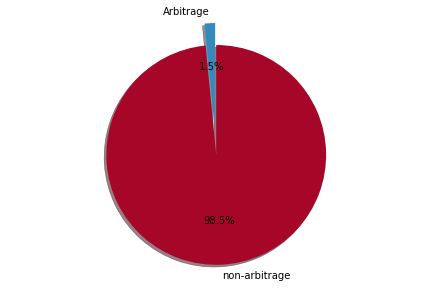
\includegraphics[width=0.32\linewidth]{figures/pie_arb}
		\caption{(left) $\alpha=0$, (middle), $\alpha=0.005$, (right) $\alpha=0.01$.}
		\label{fig:piearb0}
	\end{figure}
	
	\section{Information on traders}
	There were a total of  \textbf{7797} different traders. For visualization purposes, to avoid working with the \texttt{public id} of the user (containing a large number of characters), we assigned to each trader a unique identifier (\texttt{uid}) ranging from 0 to 7797.  We now analyze the data by each trader. A small exploratory data analysis is presented in Table \ref{tab:da2}. There, \texttt{Duration } refers to the amount of time elapsed between the first and last position of each user, \texttt{mean, min, max amount} refers to the mean, minimum and maximum amount traded by each user, \texttt{Trades} is the number of trades per user, and similarly, \texttt{Volume} is the volume traded by each user.  Once again, we can see an interesting right tail from this data; indeed for all fields, there is a rather large difference between median, mean, and max, suggesting that there are a handful of traders that are skewing these values to the right, by, e.g.,  moving larger amounts or doing a large number of trades. We investigate this in more detail next.
	
	% Please add the following required packages to your document preamble:
	% \usepackage{booktabs}
	\begin{table}[]\scriptsize{
			\begin{tabular}{@{}lllllll@{}}
				\toprule
				& Duration           & Mean amount & Min. amount & Max. amount & Trades & Volume    \\ \midrule
				mean & 12 days 22:33:45  & 790.6589     & 429.2727    & 2151.6774   & 126.5349            & 211802.9929    \\
				std  & 24 days 22:11:23  & 3026.3559    & 1694.6637   & 16923.7674  & 3191.8043           & 7143162.6203   \\
				min  & 0 days 00:00:01     & 0.0005   & 0.0000   & 0.0008   & 1.0000 & 0.0014    \\
				25\% & 0 days 00:01:29  & 76.7887  & 16.9367  & 90.2879  & 2.0000 & 279.0688  \\
				50\% & 0 days 00:20:38  & 154.9585 & 126.5936 & 160.0373 & 4.0000 & 397.9400  \\
				75\% & 15 days 02:52:58 & 326.4057 & 195.1365 & 500.0211 & 8.0000 & 1957.9870 \\
				max  & 114 days 02:59:22 & 100050.9047  & 40403.0280  & 953964.1733 & 203970.0000         & 554775886.9184 \\ \bottomrule
		\end{tabular}}
		\caption{Data analysis per user \label{tab:da2}}
	\end{table}
	
	\subsubsection*{Top traders: by number of transactions} 
	We begin by looking at the top traders by share of the number of trades ever made. In particular, we investigate those traders whose total number of transactions is larger or equal to 1\% of total transactions. We present our results in Figure \ref{fig:tradesbyprop}.  Notice how a handful of traders account for most of the transactions. We present statistics on each player in Table \ref{tab:trbp} and give a table of trader IDs in table \ref{tab:trbp_uid}. Notice, furthermore, that all players in  Table \ref{tab:trbp} have transactions that are, for the most part, arbitrages (with $\alpha=0$). It is worth mentioning that no account here was liquidated.
	
	\begin{figure}[htp]
		\centering
		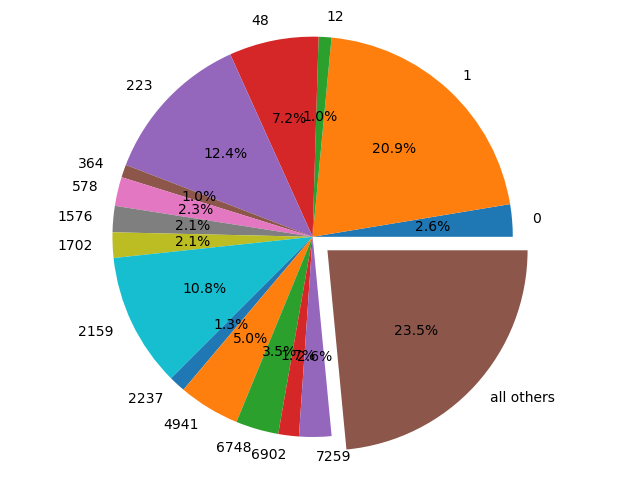
\includegraphics[width=0.7\linewidth]{figures/trades_by_prop}
		\caption{Top traders by proportion. Outer numbers represent \texttt{uid}}
		\label{fig:tradesbyprop}
	\end{figure}
	
	% Please add the following required packages to your document preamble:
	% \usepackage{booktabs}
	% Please add the following required packages to your document preamble:
	% \usepackage{booktabs}
	% Please add the following required packages to your document preamble:
	% \usepackage{booktabs}
	% Please add the following required packages to your document preamble:
	% \usepackage{booktabs}
	\begin{table}[htp]\scriptsize{
			\begin{tabular}{@{}llllllllll@{}}
				\toprule
				uid & Duration & Mean amount & Min. amount & Max amount & Prop. trades & Prop. arbs & Trades & Volume \\ \midrule
				0          & 106.901 & 1015.384 & 0.121   & 386774.777 & 0.026 & 0.614 & 25515  & 25907529.869  \\
				1          & 101.558 & 2719.890 & 171.000 & 35524.000  & 0.207 & 0.651 & 203970 & 554775886.918 \\
				12         & 94.107  & 1028.243 & 25.000  & 43976.000  & 0.010 & 0.609 & 10104  & 10389366.519  \\
				48         & 111.970 & 1052.785 & 0.001   & 18117.858  & 0.071 & 0.620 & 70580  & 74305566.494  \\
				223        & 93.652  & 1275.015 & 0.000   & 17526.977  & 0.123 & 0.633 & 121156 & 154475717.290 \\
				578        & 108.797 & 416.339  & 10.004  & 19864.414  & 0.023 & 0.611 & 22633  & 9422998.757   \\
				1576       & 94.998  & 477.946  & 10.009  & 17041.594  & 0.021 & 0.609 & 20599  & 9845211.196   \\
				1702       & 93.926  & 468.876  & 10.018  & 19864.226  & 0.020 & 0.610 & 19939  & 9348920.887   \\
				2159       & 90.292  & 1995.995 & 0.301   & 72000.000  & 0.105 & 0.622 & 103718 & 207020570.136 \\
				2237       & 84.348  & 554.681  & 10.116  & 21732.285  & 0.013 & 0.613 & 13060  & 7244140.349   \\
				4941       & 65.588  & 956.621  & 1.000   & 1004.869   & 0.049 & 0.623 & 48044  & 45959882.878  \\
				6748       & 48.619  & 1410.768 & 0.001   & 59524.675  & 0.034 & 0.631 & 33790  & 47669840.794  \\
				6902       & 50.664  & 3558.709 & 0.000   & 489199.818 & 0.016 & 0.609 & 16210  & 57686673.367  \\
				7259       & 33.477  & 3331.902 & 493.020 & 5564.551   & 0.025 & 0.613 & 25018  & 83357527.173  \\
				all others & -       & 518.567  & 0.001   & 3908.329   & 0.237 & 0.601 & 18740  & 9717949.774   \\ \bottomrule
			\end{tabular}
			\caption{Top trades by share of total trades\label{tab:trbp}}}
	\end{table}
	
	% Please add the following required packages to your document preamble:
	% \usepackage{booktabs}
	\begin{table}[]\scriptsize{
			\begin{tabular}{@{}ll@{}}
				\toprule
				uid        & user                                         \\ \midrule
				0          & 72FwbpFGoLEazJEdpqNtPNefsadUrimUqma9wSoy4qiS \\
				1          & DRKUb36Rh99NQ4CCEsZSBBfspz2vdNwM1qPY6P2jNrbu \\
				12         & 22voQuaMVuZMh1J21QHjPth5oVyAgGJV53uRsXauAsC9 \\
				48         & 8aWL3kVkJNcKuE9gkcrGf8Ewr7gv9ZKJdueBBjvfWkKH \\
				223        & 5MXwPXQC9jbFQf51EDa9sbtiuQhGWESmrLNhud4P7hBB \\
				578        & 51nJasyRr6GwVhmNoUQBgBm74p44oUPBTqZCeynMHTxW \\
				1576       & 3YNHNZ5VXntLV7YFPph4M4TJedkLBpkY2KsF5W73LZBj \\
				1702       & ASWjkz6t9pfDj6LLpEQp1pkPa4CEWnGVzNmQ3mG3GNQ4 \\
				2159       & 8vGetf9yx8CiWrM1NmCTPGyLvbwZSDz9ah3dti5hXmNV \\
				2237       & 2ss5b7W1FJw8kHiLSHQ9vBEHKavFm2a1ks3gDiopDcAA \\
				4941       & HXS9ewmRcpKZ9GCATcLYVyruCkMihcGjFdeGuycbNy2z \\
				6748       & 29oDU8LjBfnM3Xd68VeDbmJWAPW9LAZJok6dT2oMPyjy \\
				6902       & 6zMmKu29zPxzPeZLXBMV8CTdvkeqW1PECyHmPBsYH1QF \\
				7259       & 5igTNp6T23mNWTHSi4Rp9pzm5NfZ31TuFa4XMSnrQEy7 \\
				all others & 8bNgszva9WwD8JzcFezPj2hWvHNNAfdNoncAuEsgvSXT \\ \bottomrule
			\end{tabular}
			\caption{Top trades by share of total trade, user ID\label{tab:trbp_uid}}
		}
	\end{table}
	
	
	
	\subsubsection*{Top traders: by volume} 
	We repeat the previous experiment grouping traders by volume. We show our results in Figure \ref{fig:tradesbyvol} and Tables \ref{tab:tbv} and \ref{tab:tbv_ID}. Notice that our results are quite similar to those presented before. In particular, notice that the users in both groups are almost the same. This is rather unsurprisingly, however, given their trading frequency and volume, \textbf{it does suggest that these accounts might be bots.} Similarly as before,  no account here was liquidated.
	\begin{figure}
		\centering
		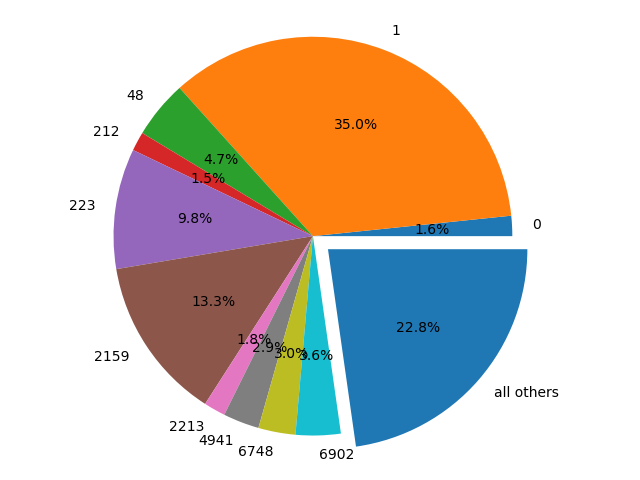
\includegraphics[width=0.7\linewidth]{figures/trades_by_vol}
		\caption{Proportion by volume. Outer numbers represent \texttt{uid}}
		\label{fig:tradesbyvol}
	\end{figure}
	
	
	\begin{table}[]\scriptsize{
			\begin{tabular}{lllllllll}
				\toprule
				uid & Duration & Mean amount & Min. amount & Max amount & Prop. volume & Prop. arbs & Trades & Volume \\ \midrule
				0    & 106.901 & 1015.384 & 0.121   & 386774.777 & 0.016 & 0.614 & 25515  & 25907529.869  \\
				1    & 101.558 & 2719.890 & 171.000 & 35524.000  & 0.336 & 0.651 & 203970 & 554775886.918 \\
				48   & 111.970 & 1052.785 & 0.001   & 18117.858  & 0.045 & 0.620 & 70580  & 74305566.494  \\
				212  & 22.206  & 8771.124 & 1.000   & 25000.000  & 0.015 & 0.594 & 2785   & 24427580.413  \\
				223  & 93.652  & 1275.015 & 0.000   & 17526.977  & 0.093 & 0.633 & 121156 & 154475717.290 \\
				2159 & 90.292  & 1995.995 & 0.301   & 72000.000  & 0.125 & 0.622 & 103718 & 207020570.136 \\
				2213 & 66.103  & 2970.977 & 1.000   & 15321.015  & 0.017 & 0.605 & 9386   & 27885588.799  \\
				4941 & 65.588  & 956.621  & 1.000   & 1004.869   & 0.028 & 0.623 & 48044  & 45959882.878  \\
				6748 & 48.619  & 1410.768 & 0.001   & 59524.675  & 0.029 & 0.631 & 33790  & 47669840.794  \\
				6902 & 50.664  & 3558.709 & 0.000   & 489199.818 & 0.035 & 0.609 & 16210  & 57686673.367  \\
				all others &-     & 3331.902     & 493.020     & 5564.551    & 0.211                          & 0.613      & 25018 & 83357527.173\\ \bottomrule
			\end{tabular}
			\caption{Top traders by volume. \label{tab:tbv}}
		}
	\end{table}
	
	% \usepackage{booktabs}
	\begin{table}[]\scriptsize{
			\begin{tabular}{@{}ll@{}}
				\toprule
				uid        & user                                         \\ \midrule
				0          & 72FwbpFGoLEazJEdpqNtPNefsadUrimUqma9wSoy4qiS \\
				1          & DRKUb36Rh99NQ4CCEsZSBBfspz2vdNwM1qPY6P2jNrbu \\
				48         & 8aWL3kVkJNcKuE9gkcrGf8Ewr7gv9ZKJdueBBjvfWkKH \\
				212        & EdMJPDmD6f3T9FtjdUZ433z1w8JHZVwQqYVkzmrG2ToK \\
				223        & 5MXwPXQC9jbFQf51EDa9sbtiuQhGWESmrLNhud4P7hBB \\
				2159       & 8vGetf9yx8CiWrM1NmCTPGyLvbwZSDz9ah3dti5hXmNV \\
				2213       & FYg8h1LKJwxtAuLqzRVTgNrbJrDjzgYAhkkgKKkWGiWm \\
				4941       & HXS9ewmRcpKZ9GCATcLYVyruCkMihcGjFdeGuycbNy2z \\
				6748       & 29oDU8LjBfnM3Xd68VeDbmJWAPW9LAZJok6dT2oMPyjy \\
				6902       & 6zMmKu29zPxzPeZLXBMV8CTdvkeqW1PECyHmPBsYH1QF \\ \bottomrule
			\end{tabular}
			\caption{Top traders by volume, ID. \label{tab:tbv_ID}}}
	\end{table}
	
	
	\subsubsection*{Liquidations}
	Lastly, we investigate liquidation and how traders behave regarding them. In particular, there were  9763 liquidations, which account for about 1\% of all trades. From a trader perspective, 919 traders got liquidated, of which 283 came back to the protocol after liquidation. A summary of statistics of those traders is presented in Table \ref{tab:liq}. I\textbf{t can be seen that most liquidated accounts were smaller ones, with a relatively small number of trades and volume}. Here, the column liquidations denote the number of liquidations suffered by an account. 
	
	\begin{table}[]\scriptsize{
			\begin{tabular}{lllllllll}
				\toprule
				& Duration & Mean amount & Min. amount & Max amount & Prop. volume & Trades      & Volume         & Liquidations   \\ \midrule
				mean & 50.021 & 1525.616 & 151.884 & 12225.002 & 0.000 & 113.636 & 154063.954 & 5.951 \\
				std  & 35.575 & 4794.715 & 814.310 & 65547.440 & 0.000 & 733.497 & 683809.624 & 6.334 \\
				min  & 0.039  & 0.002    & 0.000   & 0.002     & 0.000 & 1.000   & 0.002      & 1.000 \\
				25\% & 16.711 & 11.532   & 0.207   & 27.314    & 0.000 & 5.000   & 90.506     & 1.000 \\
				50\% & 42.081 & 116.369  & 6.001   & 497.952   & 0.000 & 13.000  & 1691.513   & 3.000 \\
				75\% & 90.209 & 642.883  & 34.902  & 2634.195  & 0.000 & 27.000  & 17761.254  & 9.000 \\
				max & 114.021     & 57898.280    & 9093.950    & 953964.173  & 0.004                          & 7638.000 & 7148023.335 & 29.000\\\bottomrule
		\end{tabular}}
		\caption{Summary statistics of liquidated accounts}\label{tab:liq}.
	\end{table} 
	\section{Oracle and mark price}\label{sec:oracle}
	
	Lastly, we investigate the relationship between oracle and mark price. We present these results in Figures \ref{fig:oraclevsmark} and \ref{fig:oraclevsmark3}. In Figure \ref{fig:oraclevsmark} (Left), we plot the historical values for oracle and mark price. As we can see, both curves have, essentially, the same behavior. However, it can be seen in a handful of regions that the mark price is above the oracle price. In Figure \ref{fig:oraclevsmar2} (Right) we plot the signed relative percentage error $\rho$ between the mark price and oracle, defined by $$\rho:=100\times\frac{\text{Oracle price}-\text{Mark price}}{\text{Oracle price}}.$$ As we can see, for the most part, the error seems to be quite small (under 5\% error), however, there are some cases where the oracle and mark price can get out of synch for much larger values. A histogram of this is presented in Figure \ref{fig:oraclevsmark3} (Left). Notice that there is a slight skew towards the left, suggesting that, consistently, the mark price is higher than the oracle price. This is further confirmed in Figure \ref{fig:oraclevsmark3} (Right). \textbf{These figures suggest that the pegging mechanism should be investigated in further detail.}
	
	\begin{figure}
		\centering
		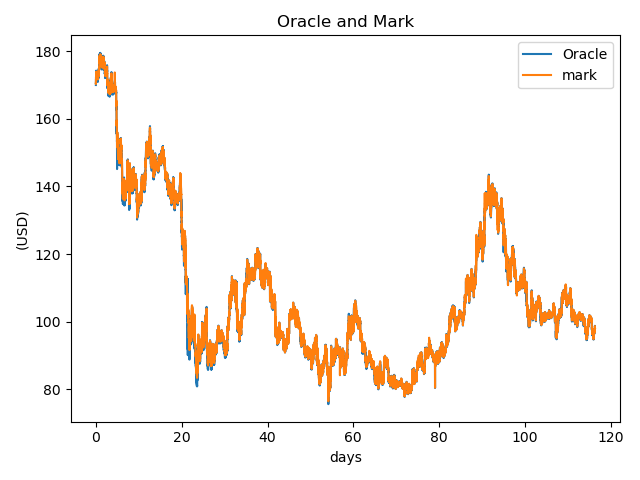
\includegraphics[width=0.47\linewidth]{figures/oracle_vs_mark}
		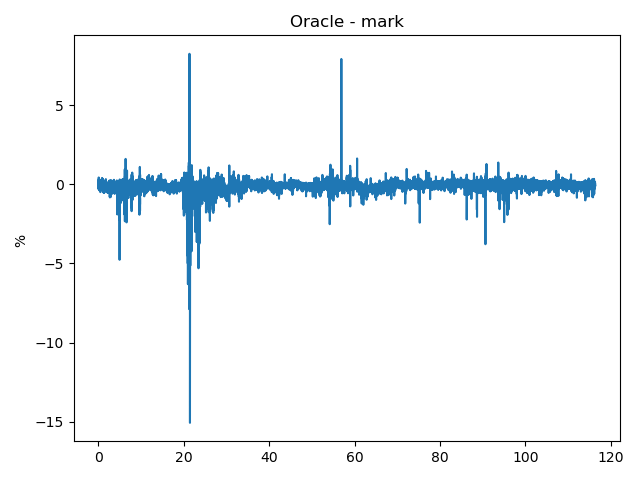
\includegraphics[width=0.47\linewidth]{figures/oracle_minus_mark}
		\caption{(Left). Oracle vs. Mark price.  (Right). Relative error, oracle vs. mark price.}
		\label{fig:oraclevsmark}
	\end{figure}
	
	
	
	\begin{figure}
		\centering
		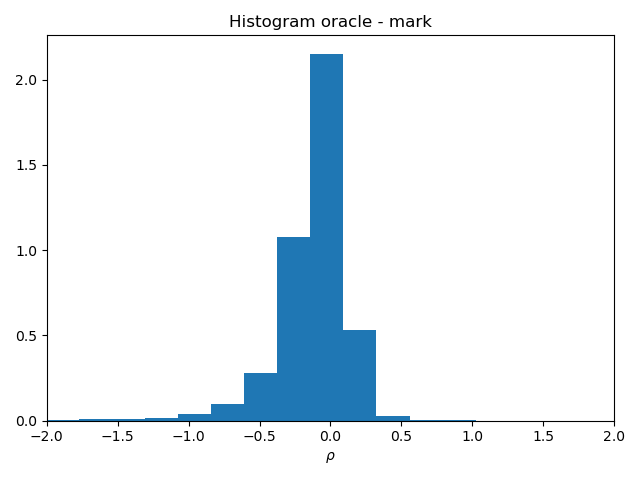
\includegraphics[width=0.47\linewidth]{figures/oracle_minus_mark_hist}
		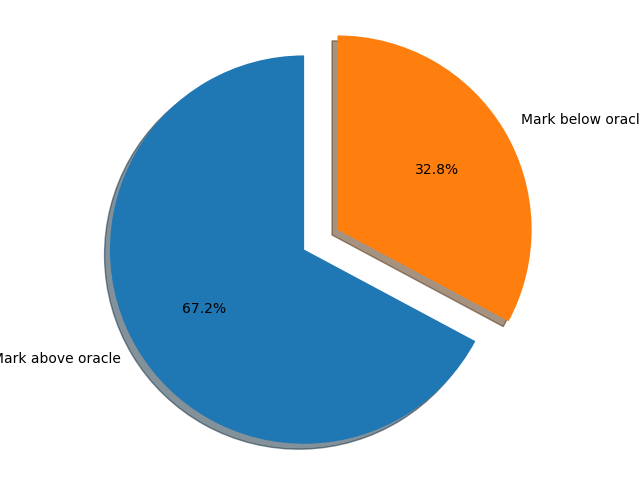
\includegraphics[width=0.47\linewidth]{figures/pie_mark_oracle}
		\caption{(Left). Histogram of relative error, oracle vs. mark price. (Right). proportion of misprice.}
		\label{fig:oraclevsmark3}
	\end{figure}
	
Lastly, we do a simple time-series analysis of the data at hand. We are interested in (i) determining the signal components and (ii) forcasting based on the time series for the oracle and mark price.  We present both results in Figures \ref{fig:fore} and \ref{fig:comps}. In particular, in Figure \ref{fig:fore}, we present the 10-day forecast for oracle price and for the difference between oracle and mark. Notice that, in either case, the fitted time series closely resembles the actual one. Notice that the fitted time series for the difference between oracle and mark price stays relatively stable around 0. The trend and seasonality components of each time series are presented in Figure \ref{fig:comps}. Interestingly enough, In either case there seem to be some distiguishable seasonality components to both time series.

 		\begin{figure}
 		\centering
 		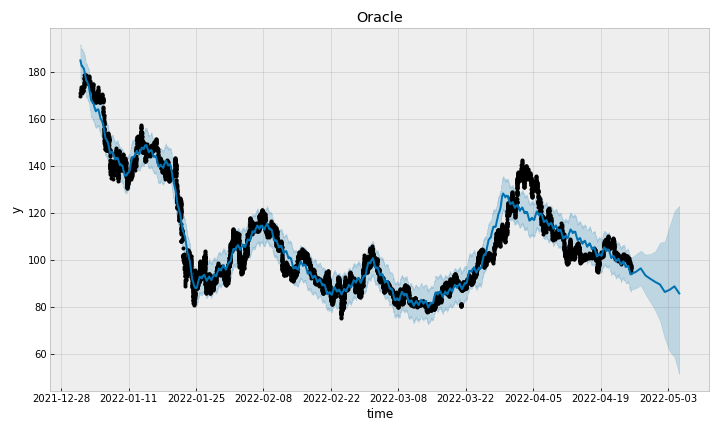
\includegraphics[width=0.7\linewidth]{figures/oracle_diff.png}
 		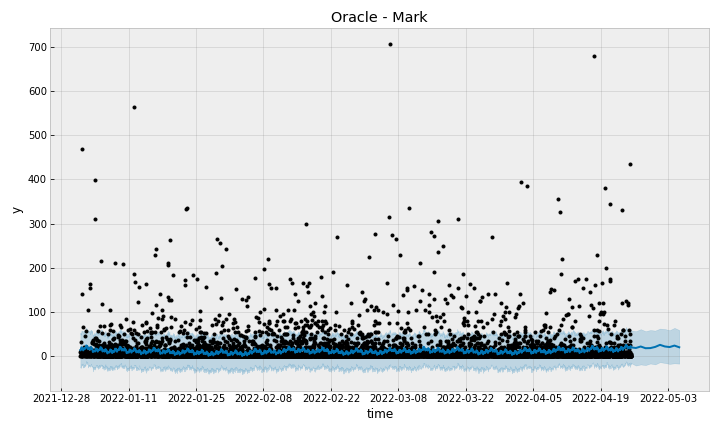
\includegraphics[width=0.7\linewidth]{figures/forecast_diff.png}
 		\caption{(Top). Forcast for the oracle price. (Bottom).  Forecast for the difference between oracle and mark price.}
 		\label{fig:fore}
 	\end{figure}
 
 
  		\begin{figure}
 	\centering
 	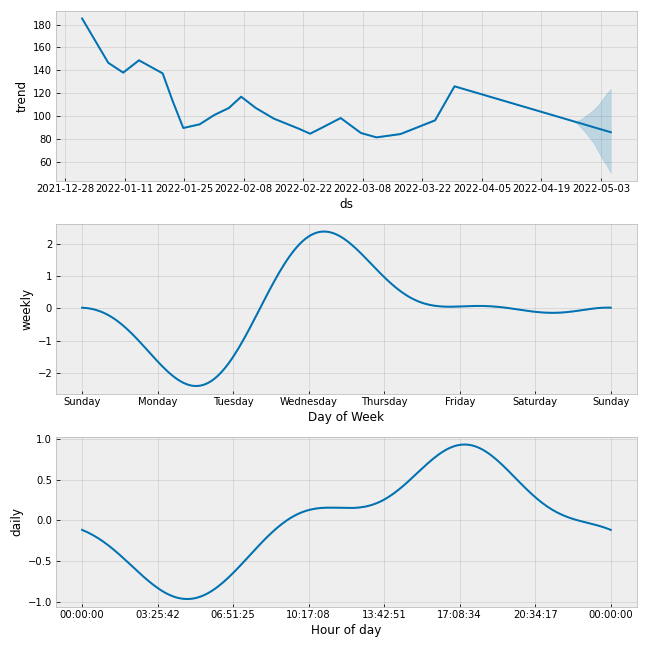
\includegraphics[width=0.47\linewidth]{figures/oracle_comps.png}
 	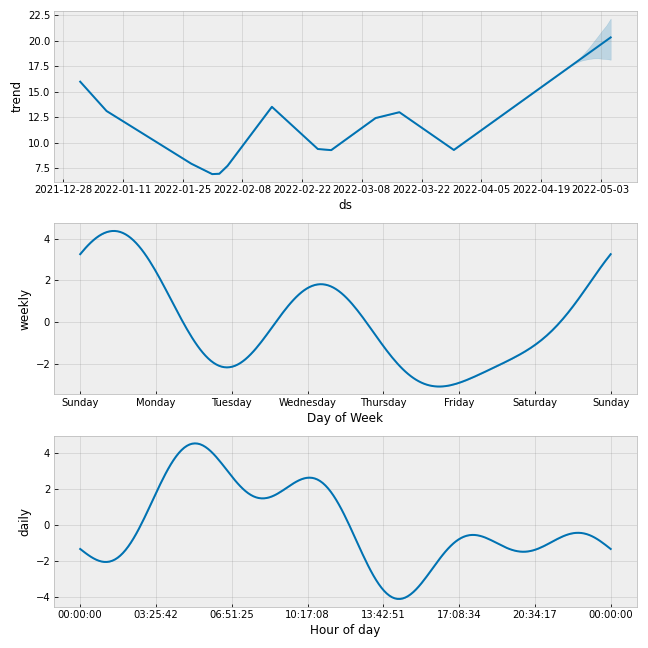
\includegraphics[width=0.47\linewidth]{figures/forecast_comps.png}
 	\caption{(Left).Components of the oracle price. (Right). Components for the difference between oracle and mark price.}
 	\label{fig:comps}
 \end{figure}
	
\end{document}          
